
\section{Généralisation aux signaux multivariés}\label{sec:sign_multivar}

\begin{definition}[Signal multivarié]\label{def:signal_multivar}
	Un \emph{signal multivarié}, ou \emph{$n-$varié}, est un vecteur composé de $n\in\N^*$ signaux $x_i$. Si $n=2$, alors on parle de signal \emph{bivarié}.
	\\
	Dans la continuité de ce qui à été dit dans la \cref{subsec:transfo_SA}, dans le cas des signaux réels, on s'intéressera au vecteur composé des transformées en SA (eq. \ref{eq:transfo_SA}, déf. \ref{def:transfo_sa&hilbert}) des $x_i$.
	\textbf{Au moins dans toute cette \namecref{sec:sign_multivar}}, un tel signal sera noté :
	\[\sa{x}(t)\ :\quad \begin{aligned} 
		\R\quad &\lr\qquad \C^n \\t\quad &\longmapsto\ \begin{pmatrix} \mathcal{A}[x_1] \\ 
			\mathcal{A}[x_2] \\ \vdots \\ \mathcal{A}[x_n] \end{pmatrix}
	\end{aligned} \]
	On supposera que chaque composante $x_i$ de $\bf{x}$ aura autant de régularité et de condition d'intégrabilité que nécessaire \textbf{(il vaudra préciser lesquelles à un moment)}.
\end{definition}

Le fait que $\bf{x}$ soit à valeur dans $\C^n$ impose un choix naturel de d'amplitude instantanée : sa norme. L'on notera alors dans tout la suite (sauf précision) :
\[\forall t\in\R,\qquad 
	\bf{x}(t) = a(t)\begin{pmatrix} a_1(t)e^{i\phi_1(t)} \\ a_2(t)e^{i\phi_2(t)} \\ \vdots \\ a_n(t)e^{i\phi_n(t)}
\end{pmatrix} \qquad\text{ avec }\qquad \big\|(a_i)_{1\leq i\leq n}\big\|=1,\quad a\geq 0
%a(t)e^{i\phi(t)}\begin{pmatrix} a_1(t)e^{i\psi_1(t)} \\ a_2(t)e^{i\psi_2(t)} \\ \vdots \\ a_n(t)e^{i\psi_n(t)}\end{pmatrix}
\]
\\
Le choix de la phase instantanée, en revanche, n'est pas plus commode. Si l'on cherche à écrire $\bf{x}$ sous la forme :
\[a(t)e^{i\phi(t)}\begin{pmatrix} a_1(t)e^{i\psi_1(t)} \\ a_2(t)e^{i\psi_2(t)} \\ \vdots \\ a_n(t)e^{i\psi_n(t)}
\end{pmatrix}\]
alors n'importe quel choix de $\phi$ est valable, il suffit que $\ \psi_i = \phi_i-\phi$.



\subsection{Phase et fréquence instantanée de signal multivarié }\label{subsec:param_instant_nvar}

Afin de contraindre ce choix, on s'inspire propriétés de la phase instantanée vu plus tôt pour en déduire deux approches :
\begin{itemize}
	\item D'une part, l'espérance de la fréquence instantanée (ici vu comme dérivée à $2\pi$ près de la phase\footnote{\itshape
		La pertinance de cette définition dans le cas multivarié sera discuté plus loin})
	doit donnée la fréquence moyenne au sens de Fourier, eq. \eqref{eq:esp_freq}.
	
	\item D'autre part, les conditions d'interprétation de la décomposition $(a_x,\phi_x)$, \cref{theo:2Bedrosian}, exige que les hautes fréquences du signal se retrouve dans la phase.
\end{itemize}

Pour cela on introduit les notations utiles au cas multivarié :
\begin{definition}[densité d’énergie]\label{def:densi_dE-mv}
Étant donné un signal multivarié $\bf{x}=(x_i)_{1\leq i\leq n}$, les densités d'énergie de chaque composante $x_i$  sont notées :
\begin{align}\label{eq:densi_dEi}
	\densit_i\ &:\quad \begin{aligned}\R\ &\lr\quad \R^+ \\ t\ &\longmapsto\ \big|x_i(t)\big|^2 = a(t)^2 a_i(t)^2 \end{aligned}  
	&
	\densis_i\ &:\quad \begin{aligned}\R\ &\lr\quad \R^+ \\ \nu\ &\longmapsto\ \big|\fou{x}_i(\nu)\big|^2 \end{aligned}
\end{align}
Et les densités d'énergies associées au signal $\bf{x}$ complet :
\begin{align}\label{eq:densi_dE-mv}
	\densit\ &:\quad \begin{aligned}\R\ &\lr\quad \R^+ \\ t\ &\longmapsto\ \big\|\bf{x}(t)\big\|^2 = \sum_{i=1}^n \densit_i(t) \end{aligned}  
	&
	\densis\ &:\quad \begin{aligned}\R\ &\lr\quad \R^+ \\ \nu\ &\longmapsto\ \big\|\fou{\bf{x}}(\nu)\big\|^2 = \sum_{i=1}^n \densis_i(t) \end{aligned}	
\end{align}
\end{definition}

La première approche, inspiré de \cite{cano_mathematical_2022} consiste donc de reprendre le ``calculation trick'' \eqref{eq:moment_f}, pour en déduire la fréquence moyenne
\begin{align*}
	\esp[\densis]{\nu} = \int_\R \nu\densis(\nu)d\nu &= \int_\R \nu\sum_{i=1}^n \densis_i(\nu) d\nu \\
		 &= \sum_{i=1}^n\esp[\densis_i]{\nu} \\
		 &= \sum_{i=1}^n\frac{1}{2\pi}\int_\R \phi_i'(t)\densit_i(t)dt \\
		 &= \frac{1}{2\pi}\int_\R a(t)^2\sum_{i=1}^n\phi_i'(t)a_i(t)^2 dt 
		 \\ &= \frac{1}{2\pi} \esp[\densit]{\sum_{i=1}^n \phi_i'{a_i}^2}
\end{align*}
\\
Ce qui mène à une première définition de la phase instantanée :
\begin{equation}\label{eq:phas_inst_v1}
	\phi = \int \sum_{i=1}^n \phi_i'(s){a_i}(s)^2ds 
	= \sum_{i=1}^n \int \phi_i'(s){a_i}(s)^2ds 
	%= \sum_{i=1}^n \esp[\nicefrac{\densit_i}{\densit}]{\phi_i'}
\end{equation}
\\

La seconde approche, fortement inspirée par les travaux de Lilly \& Olhede  \cite{lilly_analysis_2012}, se base sur la discussion autour du théorème Bedrisan sur la séparation haute-basse fréquence du signal $\bf{x}$ (\cref{subsec:Bedrisan&AM-FM}). Pour cela, l'on commence par faire apparaître la phase $\phi$ --- pour l'instant inconnue --- en écrivant $\bf{x}$ sous la forme :
\[\forall t\in\R,\qquad \bf{x}(t) = e^{i\phi(t)} e^{-i\phi(t)} \bf{x}(t) \defeq e^{i\phi(t)} \Tilde{\bf{x}}(t)\]
\\
Si $\phi$ est bien choisie, alors $\Tilde{\bf{x}}$ contient les informations associées à l'amplitude et la polarisation de $\bf{x}$. Or, la phase doit contenir les hautes fréquences du signal. 
Pour s'en assurer on demande, à l'inverse, que les basses fréquences du signal soit données par $\Tilde{\bf{x}}$ en limitant ces variations. En clair, $\phi$ doit être choisi de sorte à minimiser la dérivée $\Tilde{\bf{x}}'$ :
\[\forall t\in\R,\qquad \phi(t) = \argmin{\alpha(t)}{\big\|\Tilde{\bf{x}}'(t)\big\|_2}^2 = \argmin{\alpha(t)}{\Big\|e^{-i\alpha}\big(\bf{x}' - i\alpha'\bf{x}\big)\Big\|_2}^2 = \argmin{\alpha(t)}{\big\|\bf{x}' - i\alpha'\bf{x}\big\|_2}^2\]
\\
La contrainte ne dépendant que de la dérivée $\alpha'$, on se ramène à :
\[\min_{\alpha(t)}{\|\Tilde{\bf{x}}'(t)\|_2}^2 = \min_{\alpha'(t)}{\big\|\bf{x}'(t) - \alpha'(t) \bf{x}(t)\big\|_2}^2\]
\\
En rappelant que $\frac{d}{dx}{\big\|f(x)\big\|_2}^2 = 2\Re e\big\langle f(x), f'(x)\big\rangle$, il vient que ce minimum\footnote{\itshape
	L'extremum obtenu est l'unique minimum puisque $t\longmapsto \|at + b\|^2$ est strictement convexe pour $a\neq0$.}
 est atteint par $\phi'(t)$ à condition que :
\begin{align*}
	\frac{d}{d\phi'}{\big\| \bf{x}' - i\phi' \bf{x}\big\|_2}^2 = 0 \quad \Llr\quad
		0 &= 2\Re e\left\langle  \bf{x}' - i\phi' \bf{x} ,  \frac{d}{d\phi'}\big(\bf{x}' - i\phi' \bf{x}\big)\right\rangle \\
		&= 2\Re e\big\langle  \bf{x}' - i\phi' \bf{x} ,  - i \bf{x}\big\rangle \\
		&= 2\Re e\Big(i\big\langle  \bf{x}' ,  \bf{x}\big\rangle\Big) + 2\phi'\Re e\big\langle   \bf{x} ,  \bf{x}\big\rangle\\
		&= -2\Im m\big\langle  \bf{x}' ,  \bf{x}\big\rangle + 2\phi'{\| \bf{x}\|_2}^2
\end{align*}
Ainsi :
\begin{align}\label{eq:phas_inst_v2}
	\phi' &= \frac{\Im m\big\langle  \bf{x}' ,  \bf{x}\big\rangle}{{\| \bf{x}\|_2}^2} = \frac{-\Im m\big\langle  \bf{x},  \bf{x}'\big\rangle}{{\| \bf{x}\|_2}^2}  &  &\text{et}  &  \phi &= -\Im m\int \frac{\big\langle \bf{x}(s) , \bf{x}'(s) \big\rangle}{\|\bf{x}(s)\|^2} ds
\end{align}
\\
Ce qui, sous forme exponentiel, se réécrit :
\begin{align*}
	-\Im m\frac{\big\langle \bf{x}(t) , \bf{x}'(t) \big\rangle}{\|\bf{x}(t)\|^2} &= -\Im m\frac{1}{a(t)^2} \sum_{i=1}^n a(t)a_i(t)e^{i\phi_i(t)}\congu{\Big( \big(aa_i\big)'(t) +a(t)a_i(t)i\phi_i'(t)\Big)e^{i\phi_i(t)}} \\
	&= -\Im m\frac{1}{a(t)^2} \sum_{i=1}^n a(t)a_i(t)\big(aa_i\big)'(t) -ia(t)^2a_i(t)^2\phi_i'(t) \\
	&= -\frac{1}{a(t)^2} \sum_{i=1}^n -a(t)^2a_i(t)^2 \phi_i'(t) \\
	&= \sum_{i=1}^n a_i(t)^2 \phi_i'(t)
\end{align*}
Soit la même expression que \eqref{eq:phas_inst_v1} obtenue par le premier raisonnement.
\\
\begin{remarque}[Notation à reprendre ($aa_i$)]
	Toujours avec les mêmes notations, une conséquence de l'\cref{eq:phas_inst_v2} est que les fréquences $\psi_i$ restantes sont de moyenne nulle dans le sens où :
	\begin{equation}\label{eq:sum_esp_null}
		\sum_{i=1}^n \int \psi_i'(s){a_i}(s)^2ds =0
	\end{equation}
	Moralement, ca revient juste à dire qu'en définissant $\phi$ suivant Lilly, on a ôté au $\psi_i$ la phase moyenne pondérée et donc, tout naturellement, les nouvelles phase individuelles $\psi_i$ sont centrés (à la même pondération près). Cela revient peut ou prou à la première \cref{eq:phas_inst_v1}.
	\\
	Pour le montrer, il suffit de refaire le calcul de la phase instantanée :
	\begin{align*}
		\big\langle \bf{x}(t) \,|\, \dot{\bf{x}}(t) \big\rangle &= \Big\langle \Big(a_i(t)e^{i(\phi(t)+\psi_i(t))}\Big)_i \,\Big|\, \Big(\big(a_i'(t)+i\big( \phi(t)+\psi_i(t) \big)a_i(t)\big)e^{i(\phi(t)+\psi_i(t))}\Big)_i \Big\rangle \\
		&= \sum_i a_i(t) \Big(a_i'(t)-i\big(\phi'(t) + \psi_i'(t)\big)a_i(t)\Big) \\
		&= \sum_i a_i(t)a_i'(t)-i\sum_i \big(\phi'(t) + \psi_i'(t)\big)a_i(t)^2 \\
		&= \sum_i a_i(t)a_i'(t)-i \phi'(t)\sum_ia_i(t)^2  - i\sum_i \psi_i'(t)a_i(t)^2 \\
		&= \sum_i a_i(t)a_i'(t)-i \phi'(t)\big\|a(t)\big\|^2  - i\sum_i \psi_i'(t)a_i(t)^2
	\end{align*}
	\\
	Ce qui mène à :
	\begin{align*}
		\phased(\bf{x},t_0,t) &= \int_{t_0}^t \frac{\varphi'(s)\big\|a(s)\big\|^2}{\big\|a(s)\big\|^2} ds  + \sum_i\int_{t_0}^t \frac{\varphi_i'(s)a_i(s)^2}{\big\|a(s)\big\|^2} ds \\
		&=\phased(\bf{x},t_0,t)  + = \sum_{i=1}^n \int \psi_i'(s){a_i}(s)^2ds 
	\end{align*}
\end{remarque}




\subsection{Cas bivarié et trivarié}

\subsubsection{Bivarié}

\begin{proposition}[phases de signal AM--FM--PM]\label{prop:phased/t_2var}
	\'Etant donné un signal bivarié AM--FM--PM $\bf{x}$, \ie~de la forme :
	\begin{equation}\label{eq:exp_elliptik_2var}
		\bf{x} = ae^{i\varphi} R_{\theta} \begin{pmatrix} \cos\chi \\ -i\sin\chi \end{pmatrix} 
			= a(t)e^{i\varphi} \begin{pmatrix} \cos\theta \cos\chi + i\sin\theta \sin\chi \\ \sin\theta \cos\chi - i\cos\theta \sin\chi \end{pmatrix}
	\end{equation}
	\\
	la phase dynamique de $\bf{x}$ est donnée par :
	\begin{equation}\label{eq:phased_2var}
		\phased(\bf{x}, t_0,t) = \int_{t_0}^t \dot{\varphi}(s) + \dot{\theta}(s) \sin2\chi(s) ds = \varphi(t) -\varphi(t_0) + \int_{t_0}^t\dot{\theta}(s) \sin2\chi(s) ds
	\end{equation}
	\\
	Soit une différence de phase $\varphi$ mais avec un terme en plus. Donc $\varphi$ ne doit (\textbf{doit?}) pas être interpréter comme la phase instantanée du signal, où du moins pas au sens donnée dans la \cref{subsec:param_instant_nvar}.
	\\
	La phase totale, elle, s'écrit :
	\begin{equation}\label{eq:phaset_2var}
		\begin{aligned}
			\phaset(\bf{x},t_0,t) = \arg\big\langle \bf{x}(t), \bf{x}(t_0)\big\rangle &= \varphi(t)-\varphi(t_0) + \arg\Big(\cos\Delta\theta \cos\Delta\chi + i\sin\Delta\theta \sin\big(\chi(t_0)+\chi(t)\big)\Big) \\
			&= \varphi(t)-\varphi(t_0) + \arctan\left(\tan\Delta\theta \frac{ \tan\chi(t_0)+\tan\chi(t)}{1 + \tan\chi(t_0)\tan\chi(t)}\right)
		\end{aligned}
	\end{equation}
	ou $\ \Delta y = y(t) - y(t_0)\ $ pour $\ y=\varphi,\theta,\chi$. \textbf{(adapte signe démo)}
\end{proposition}

\begin{demo}[de la \cref{prop:phased/t_2var}]
	Par souci de lisibilité, on note $\mathcal{U} = R_{\theta} \begin{pmatrix} \cos\chi \\ -i\sin\chi \end{pmatrix}$ de sorte que la dérivée de $\bf{x}$ s'écrive :
	\begin{align*}
		\dot{\bf{x}} 
			&= \dot{a}e^{i\varphi}\mathcal{U} + ia\dot{\varphi}e^{i\varphi} \mathcal{U} + ae^{i\varphi}\dot{\theta}\begin{pmatrix} -\sin\theta \cos\chi + i\cos\theta \sin\chi \\ \cos\theta \cos\chi + i\sin\theta \sin\chi \end{pmatrix} + ae^{i\varphi}\dot{\chi}\begin{pmatrix} -\cos\theta \sin\chi + i\sin\theta \cos\chi \\ -\sin\theta \sin\chi - i\cos\theta \cos\chi \end{pmatrix} \\
			&= \dot{a}e^{i\varphi}\mathcal{U} + ia\dot{\varphi}e^{i\varphi} \mathcal{U} + ae^{i\varphi}\dot{\theta}\begin{pmatrix} 0 & -1 \\ 1 & 0 \end{pmatrix}\mathcal{U} + ae^{i\varphi}\dot{\chi}\begin{pmatrix} 0 & i \\ -i & 0 \end{pmatrix}\congu{\mathcal{U}}
	\end{align*}
	\\
	Le produit hermitien $\langle \bf{x}, \dot{\bf{x}}\rangle$ s'écrit alors :
	\begin{align*}
		\langle \bf{x}, \dot{\bf{x}}\rangle 
			&= \left\langle ae^{i\varphi}\mathcal{U}, \dot{a}e^{i\varphi}\mathcal{U} + ia\dot{\varphi}e^{i\varphi} \mathcal{U} + ae^{i\varphi}\dot{\theta}\begin{pmatrix} 0 & -1 \\ 1 & 0 \end{pmatrix}\mathcal{U} + ae^{i\varphi}\dot{\chi}\begin{pmatrix} 0 & i \\ -i & 0 \end{pmatrix}\congu{\mathcal{U}}\right\rangle \\
			&= \left\langle a\mathcal{U}, \dot{a}\mathcal{U} + ia\dot{\varphi} \mathcal{U} + a\dot{\theta}\begin{pmatrix} 0 & -1 \\ 1 & 0 \end{pmatrix}\mathcal{U} + a\dot{\chi}\begin{pmatrix} 0 & i \\ -i & 0 \end{pmatrix}\congu{\mathcal{U}}\right\rangle \\
			&= a\dot{a} \big\langle \mathcal{U}, \mathcal{U}\big\rangle  - ia^2\dot{\varphi} \big\langle \mathcal{U}, \mathcal{U}\big\rangle  + a^2\dot{\theta}\left\langle \mathcal{U}, \begin{pmatrix} 0 & -1 \\ 1 & 0 \end{pmatrix}\mathcal{U}\right\rangle + ia^2\dot{\chi}\left\langle \mathcal{U}, \begin{pmatrix} 0 & -1 \\ 1 & 0 \end{pmatrix}\congu{\mathcal{U}}\right\rangle
	\end{align*}
	où les deux derniers produits hermitiens donnent :
	\begin{align*}
		\left\langle \mathcal{U}, \begin{pmatrix} 0 & -1 \\ 1 & 0 \end{pmatrix}\mathcal{U}\right\rangle &= -\mathcal{U}_1\congu{\mathcal{U}_2} + \mathcal{U}_2\congu{\mathcal{U}_1} \\
		&= 2i\Im m\big(\congu{\mathcal{U}_1} \mathcal{U}_2\big) \\
		&= 2i\Im m\big(\cos\theta \cos\chi - i \sin\theta \sin\chi \big) \big( \sin\theta \cos\chi - i \cos\theta \sin\chi \big) \\
		&= 2i\big(-\cos^2\theta \cos\chi \sin\chi - \sin^2\theta \sin\chi \cos\chi \big) \\
		&= -2i\big( \cos\chi \sin\chi + \sin\chi \cos\chi \big) \\
		&= -i\sin2\chi 
		\\ \\
	\left\langle \mathcal{U}, \begin{pmatrix} 0 & -1 \\ 1 & 0 \end{pmatrix}\congu{\mathcal{U}}\right\rangle &= -\mathcal{U}_1\mathcal{U}_2 + \mathcal{U}_2\mathcal{U}_1 = 0
	\end{align*}
	\\
	D'où, sachant que $\ \|\bf{x}\|^2=a^2\ $ et $\ \|\mathcal{U}\|=1$, la formule :
	\begin{align*}
		-\frac{\Im m\big\langle \bf{x},\dot{\bf{x}}\big\rangle}{\|\bf{x}\|^2} &= -\frac{1}{a^2}\Im m\Big(a\dot{a} \big\langle \mathcal{U}, \mathcal{U}\big\rangle  - ia^2\dot{\varphi} \big\langle \mathcal{U}, \mathcal{U}\big\rangle - ia^2\dot{\theta} \sin2\chi \Big) \\
		&= \frac{1}{a^2} \Big( a^2\dot{\varphi} \|\mathcal{U}\|^2 + a^2\dot{\theta} \sin2\chi \Big) \\
		&= \dot{\varphi} + \dot{\theta} \sin2\chi
	\end{align*}
	%\begin{pmatrix} \cos\theta \cos\chi + i\sin\theta \sin\chi \\ \sin\theta \cos\chi - i\cos\theta \sin\chi \end{pmatrix}
	\\
	
	Pour la phase totale, on note cette fois $\mathcal{V} = \begin{pmatrix} \cos\chi \\ -i\sin\chi \end{pmatrix}$ et on a :
	\begin{align*}
		\big\langle \bf{x}(t_0), \bf{x}(t)\big\rangle &= \Big\langle a(t_0)e^{i\varphi(t_0)}R_{\theta(t_0)}\mathcal{V}(t_0), a(t)e^{i\varphi(t)}R_{\theta(t)}\mathcal{V}(t) \Big\rangle \\
		&= a(t_0)e^{i\varphi(t_0)}a(t)e^{-i\varphi(t)}\Big\langle R_{\theta(t_0)}\mathcal{V}(t_0), R_{\theta(t)}\mathcal{V}(t) \Big\rangle \\
		%&= a(t_0)a(t)e^{i(\varphi(t_0)-\varphi(t))}\Big\langle \mathcal{V}(t_0), R_{\theta(t_0)}^{-1}R_{\theta(t)}\mathcal{V}(t) \Big\rangle \\
		&= a(t_0)a(t)e^{i(\varphi(t_0)-\varphi(t))}\Big\langle \mathcal{V}(t_0), R_{\theta(t)- \theta(t_0)}\mathcal{V}(t) \Big\rangle
	\end{align*}
	Pour alléger les notations, on note $\ \Delta y =y(t)-y(t_0)$, $\ y_1=y(t_0)\ $ et $\ y_2=(t)\ $ pour $\ y=\varphi,\theta,\chi$. Le produit hermitien à droite s'écrit alors :
	\begin{align*}
		\Big\langle \mathcal{V}(t_0), R_{\Delta\theta}\mathcal{V}(t) \Big\rangle &= \begin{pmatrix} \cos\chi_1 & -i\sin\chi_1 \end{pmatrix}  \begin{pmatrix} \cos\Delta\theta \cos\chi_2 - i\sin\Delta\theta \sin\chi_2 \\ \sin\Delta\theta \cos\chi_2 + i\cos\Delta\theta \sin\chi_2 \end{pmatrix} \\
		&= \cos\chi_1\Big(\cos\Delta\theta \cos\chi_2 - i\sin\Delta\theta \sin\chi_2\Big) - i\sin\chi_1\Big(\sin\Delta\theta \cos\chi_2 + i\cos\Delta\theta \sin\chi_2\Big) \\
		&= \cos\Delta\theta \Big(\cos\chi_1 \cos\chi_2 + \sin\chi_1 \sin\chi_2\Big) - i\sin\Delta\theta \Big( \cos\chi_1 \sin\chi_2 + \sin\chi_1\cos\chi_2\Big) \\
		&= \cos\Delta\theta \cos\Delta\chi - i\sin\Delta\theta \sin(\chi_1+\chi_2)
	\end{align*}
\end{demo}




\subsubsection{Trivarié}

\begin{itemize}
	\item Version de Lilly \cite{lilly_modulated_2011}
	\begin{equation}
		\begin{aligned}
			\sa{\bf{x}}(t) &= e^{i\phi(t)} R_1\big(\alpha(t)\big)\ R_3\big(\beta(t)\big)\ R_1\big(\theta(t)\big)\begin{pmatrix}
				a(t) \\ -ib(t) \\ 0
			\end{pmatrix} \\
			&= a(t)e^{i\phi(t)} R_1\big(\alpha(t)\big)\ R_3\big(\beta(t)\big)\ R_1\big(\theta(t)\big)\begin{pmatrix}
				\cos\chi(t) \\ -i\sin\chi(t) \\ 0
			\end{pmatrix}
		\end{aligned}
	\end{equation}
	
	\begin{align*}
		&\text{avec : }  &  
		R_1(\theta) &= \begin{pmatrix}
			1 & 0 & 0 \\ 0 & \cos\theta & -\sin\theta \\ 0 & \sin\theta & \cos\theta
		\end{pmatrix}  &  
		R_3(\theta) &= \begin{pmatrix}
			\cos\theta & -\sin\theta & 0 \\ \sin\theta & \cos\theta & 0 \\ 0 & 0 & 1 
		\end{pmatrix}
	\end{align*}
	
	Donc une amplitude / phase instantanée $A$ / $\phi$ et une polarisation instantanée d'ellipse paramétrée par $\chi$ et orientée par la rotation $R_1R_3R_1$.
	
	\item On note d'abord que (Lefevre \cite{lefevre_polarization_2021}) :
	\[\begin{pmatrix}
		\cos\chi(t) \\ -i\sin\chi(t) \\ 0
	\end{pmatrix} = \begin{pmatrix}
		\cos\chi(t) & i\sin\chi(t) & 0 \\ -i\sin\chi(t) & \cos\chi(t) & 0 \\ 0 & 0 & 1
	\end{pmatrix}\begin{pmatrix}
	1 \\ 0 \\ 0
	\end{pmatrix}\]
	Ce qui, en terme de matrice de Gall-man $(\lambda_i)$ (généralisation de la base de Pauli à $\U{3}$), devient :
	\begin{align*}
		\sa{\bf{x}}(t) &= a(t)e^{i\phi(t)} R_1\big(\alpha(t)\big)\ R_3\big(\beta(t)\big)\ R_1\big(\theta(t)\big)\begin{pmatrix}
			\cos\chi(t) \\ -i\sin\chi(t) \\ 0
		\end{pmatrix} \\
		&= a(t)e^{i\phi(t)} e^{i\alpha \lambda_7} e^{i\beta \lambda_3} e^{i\theta \lambda_7} e^{-i\chi \lambda_1}\begin{pmatrix}
			1 \\ 0 \\ 0
		\end{pmatrix}
	\end{align*}
	
	
\end{itemize}





\subsection{Généralisation de ces formules au cas $\bf{n-}$varié}\label{subsec:phase_instant}

\begin{proposition}[phase de signal AM--FM--PM $n$-varié]\label{prop:phased_nvar}
	La formule \eqref{eq:phased_2var} de la \cref{prop:phased/t_2var} ce généralise très bien à plus haute dimension. En écrivant $\bf{x}$ sous la forme :
	\begin{align}\label{eq:exp_elliptik_nvar}
		\bf{x}(t) &= a(t)e^{i\varphi} R_{\Theta(t)} \mathcal{V}(t)  &  \text{où }\ R_{\Theta(t)} \in\SO_n(\R)  \ \text{ et }\  \mathcal{V}(t) &= \begin{pmatrix} \cos\chi(t) \\ -i\sin\chi(t) \\ 0 \\ \vdots \\ 0 \end{pmatrix}
	\end{align}
	\\
	la phase dynamique de $\bf{x}$ est donnée par :
	\begin{equation}\label{eq:phased_nvar-v1}
		\begin{aligned}
			\phased(\bf{x}, t_0,t) &= \int_{t_0}^t \dot{\varphi}(s) + \sin2\chi \big\langle \Tilde{R}_{\Theta(s)} e_1, e_2\big\rangle ds \\
			&= \varphi(t) -\varphi(t_0) + \int_{t_0}^t \sin2\chi \big\langle \Tilde{R}_{\Theta(s)} e_1, e_2\big\rangle ds
		\end{aligned}
	\end{equation}
	où $e_j=\delta^i_j\in\R^n$ et $\Tilde{R}_{\Theta(t)}$ est la matrice anti-symétrique :
	\[\Tilde{R}_{\Theta(t)} =\, ^tR_{\Theta(t)} \dot{R}_{\Theta(t)}\in\mathcal{A}_n(\R)\]
	\\
	En récrivant $R_\Theta$ comme composition d'une rotation $R_\Lambda$ et d'une rotation $R_\theta$ de l'ellipse dans son plan, \ie~:
	\[R_\Theta = R_\Lambda R_\theta = R_\Lambda \begin{pmatrix}\cos\theta & -\sin\theta \\ \sin\theta & \cos\theta \\ & & \mathbb{O}_{n-2}
	\end{pmatrix}\]
	alors la phase dynamique ce réécrit encore :
	\begin{equation}\label{eq:phased_nvar-v2}
		\phased(\bf{x}, t_0,t) = \varphi(t) -\varphi(t_0) + \int_{t_0}^t \dot{\theta}(s) \sin2\chi(s) ds + \int_{t_0}^t \sin2\chi(s) \big\langle \Tilde{R}_{\Lambda(s)} \Tilde{e}_1(s),  \Tilde{e}_2(s)\big\rangle ds
		%= \varphi(t) -\varphi(t_0) + \int_{t_0}^t  \Big(\dot{\theta}(s) + \big\langle \dot{R}_{\Lambda(s)} \Tilde{e}_1, R_{\Lambda(s)} \Tilde{e}_2\big\rangle \Big) \sin2\chi(s) ds
	\end{equation}
	où cette fois $\Tilde{e}_1$ (resp. $\Tilde{e}_1$) donne la direction du demi-grand (resp. -petit) axe de l'ellipse paramétrée par $\chi$ :
	\begin{align*}
		 \Tilde{e}_1 &= R_\theta e_1  &   \Tilde{e}_2 &= R_\theta e_2
	\end{align*}
\end{proposition}

\begin{demo}
	D'abord, on a la différentielle :
	\begin{align*}
		\dot{\bf{x}} = \frac{d}{dt}\Big(a e^{i\varphi}R_{\Theta} \mathcal{V}\Big) &= \dot{a}e^{i\varphi}R_{\Theta} \mathcal{V} + ia\dot{\varphi}e^{i\varphi} R_{\Theta} \mathcal{V} + ae^{i\varphi}\dot{R}_{\Theta}\mathcal{V} + ae^{i\varphi}R_\Theta\dot{\mathcal{V}} \\
		&= \big(\dot{a} + ia\dot{\varphi}\big)e^{i\varphi}R_{\Theta} \mathcal{V} + ae^{i\varphi}\Big(\dot{R}_{\Theta}\mathcal{V} + R_\Theta\dot{\mathcal{V}}\Big)
	\end{align*}
	où le vecteur $\dot{\mathcal{V}}$ se réécrit :
	\begin{align*}
		\dot{\mathcal{V}} = \frac{d}{dt}\begin{pmatrix}
			\cos\chi \\ -i\sin\chi \\ 0 \\ \vdots \\ 0 
		\end{pmatrix} = \dot{\chi}\begin{pmatrix}
			-\sin\chi(t) \\ -i\cos\chi \\ 0 \\ \vdots \\ 0 
		\end{pmatrix} = i \dot{\chi} \begin{pmatrix}
			0 & 1 \\ 1 & 0 \\ & & \mathbb{O}_{n-2}
		\end{pmatrix}\begin{pmatrix} 
			\cos\chi \\ -i\sin\chi \\ 0 \\ \vdots \\ 0 
		\end{pmatrix} \defeq i\dot{\chi}J\mathcal{V}
	\end{align*}
	On en déduit alors :
	\begin{align*}
			-\frac{\Im m\big\langle \bf{x},\dot{\bf{x}}\big\rangle}{\|\bf{x}\|^2} &= -\frac{1}{\|\bf{x}\|^2}\Im m \left\langle ae^{i\varphi}R_\Theta \mathcal{V},  \big(\dot{a} + ia\dot{\varphi}\big)e^{i\varphi}R_{\Theta} \mathcal{V} + ae^{i\varphi}\Big(\dot{R}_{\Theta}\mathcal{V} + i\dot{\chi}R_\Theta J\mathcal{V}\Big)\right\rangle \\
			&= \dot{\varphi} + \Im m \left\langle R_\Theta \mathcal{V},   \dot{R}_{\Theta}\mathcal{V}\right\rangle + \Im m \Big( i\dot{\chi} \big\langle R_\Theta \mathcal{V}, R_\Theta J\mathcal{V}\big\rangle \Big) \\
			&= \dot{\varphi} + \Im m \left\langle R_\Theta \mathcal{V},   \dot{R}_{\Theta}\mathcal{V}\right\rangle + \dot{\chi} \Re e \big\langle \mathcal{V}, J\mathcal{V}\big\rangle
	\end{align*}
	\\
	On montre, avec un calcul similaire à la démonstration de la \cref{prop:phased/t_2var}, que le dernier terme est nul. Le deuxième terme, lui, ce réécrit en fonction de la base canonique $(e_i)$ de $\R^n$ :
	\begin{align*}
		\left\langle R_\Theta \mathcal{V},   \dot{R}_{\Theta}\mathcal{V}\right\rangle 
		&= \left\langle R_\Theta (\cos\chi e_1 -i\sin\chi e_2),   \dot{R}_{\Theta}(\cos\chi e_1 -i\sin\chi e_2)\right\rangle  \\
		&= \cos^2\chi \left\langle R_\Theta  e_1 ,   \dot{R}_{\Theta}e_1\right\rangle  + \sin^2\chi \left\langle R_\Theta e_2,   \dot{R}_{\Theta}e_2\right\rangle  
		- i \cos\chi  \sin\chi \left(\left\langle R_\Theta e_1,   \dot{R}_{\Theta} e_2\right\rangle - \left\langle R_\Theta e_2,   \dot{R}_{\Theta}e_1 \right\rangle\right) 
	\end{align*}

	Notons à présent que comme $R_{\Theta(t)}\in\SO_n(\R)$, la différentielle $\dot{R}_{\Theta}$ est à valeur dans le fibré tangent $\tg{\SO_n(\R)}$. Sachant que $\tg[\Theta(t)]{\SO_n(\R)} = R_{\Theta(t)}\asym{n}$, la différentielle $\dot{R}_\Theta$ s'écrit :
	\[\forall t\in\R,\quad \dot{R}_{\Theta(t)}\in \tg[\Theta(t)]{\SO_n(\R)}\ \Llr\ \exists \Tilde{R}_{\Theta(t)}\in\asym{n}\ |\ \dot{R}_{\Theta(t)} = R_{\Theta(t)} \Tilde{R}_{\Theta(t)}\]
	\\
	Cela permet d'écrire :
	\begin{align*}
		-\frac{\Im m\big\langle \bf{x},\dot{\bf{x}}\big\rangle}{\|\bf{x}\|^2} = \dot{\varphi} + \Im m \left\langle R_\Theta \mathcal{V},   \dot{R}_{\Theta}\mathcal{V}\right\rangle %+ \dot{\chi} \Re e \big\langle \mathcal{V}, J\mathcal{V}\big\rangle 
		&= \dot{\varphi} -  \cos\chi \sin\chi \left(\left\langle R_\Theta e_1,   \dot{R}_{\Theta} e_2\right\rangle - \left\langle R_\Theta e_2,   \dot{R}_{\Theta}e_1 \right\rangle\right) \\
		&= \dot{\varphi} - \frac{1}{2} \sin2\chi \left(\left\langle e_1,   \Tilde{R}_{\Theta} e_2\right\rangle - \left\langle \, ^t\Tilde{R}_\Theta e_2, e_1 \right\rangle\right) \\
		&= \dot{\varphi} - \sin2\chi \left\langle e_1, \Tilde{R}_{\Theta} e_2\right\rangle \\
		&= \dot{\varphi} + \sin2\chi \left\langle \Tilde{R}_{\Theta} e_1,  e_2\right\rangle
	\end{align*}
\end{demo}


\begin{itemize}
	\item Les quaternions ça ce généralise trop mal (au dessus c'est les octinions, c'est un calvaire et ca va pas plus loin)
	
	\item Ca peut s'écrire en terme d'algèbre de Cliffor (Lefevre \cite{lefevre_polarization_2021})... pas dingue non plus (pb de dimension principalement)
	
	\item Les bases de $\U{n}$ parait être le meilleur choix mais on a pas de ``bonne base'' pour de plus haute dimension.
	
	\item question : est-ce qu'on en a besoin pour la phase géométrique ? (transi vers une formulation géo diff-like ?)
\end{itemize}




\section{Notes sur l'approche Géométrique}

\subsection{Le plan du mémoire (trop long)}

\begin{enumerate}[label=\Roman* --- ]
	
	\item Introduction du phénomène 
	\begin{enumerate}[label=\arabic* --- ]
		
		\item ``En phase'' de Pancharatnam
		
		\item Dessin de Bohm
		\begin{itemize}
			
			\item cas cyclique (plus intéressant qu'adiabatique)
			
			\item cadre quantique, on a Schrödonger \eqref{eq:schrodinger}
			
			\item Explique le dessin de Bohm \cref{fig:2lifts}
			
			\item Ils font un peu de géo diff \cite{mukunda_quantum_1993,bohm_geometric_2003} mais nous on veut écrire ca propre
		\end{itemize}
		
		\item On veut une description géo diff, on a besoin de quoi ?
		\begin{itemize}
			
			\item passage en complexe
			
			\item Espace : $\U{1}\times\PC{n}$
			
			\item fibré principal 
			
			\item connexion
			
			 \item holonomie
		\end{itemize}
	\end{enumerate}
		
	\item Préliminaire
	\begin{enumerate}[label=\arabic* --- ]
		
		\item Transformation en SA
		
		\item Un peu de géo diff 
		\begin{enumerate}[label=\arabic{enumi}.\arabic* --- ]
			
			%\item Formes différentielles
			
			\item Variété complexe
			
			\item Holonomie et Bonnet-Gauss
			
			\item Fibré principaux
			\begin{itemize}
				\item variété fibrée
				
				\item fibré principal
				
				\item esapce tangent
				
				\item --- verticaux et horizontaux
				
				\item --- connexion vie métric
				
				\item ``universal $\U{1}$ principal bundle''
			\end{itemize}
			
			\item Connexion
			\begin{itemize}
				\item Connexion sur fibré principal
				
				\item Connexion sur variété/fibré tangent (Levi-Civita)
				
				\item Lien entre les deux
				
				\item Courbure de la connexion ?
			\end{itemize}
			
			\item Espace $\PC{n}$
			\begin{itemize}
				\item ``universal $\U{1}$ principal bundle''
				
				\item Connexion de Fubini-Study
				
				\item Séparation Fisher/phase géo
				
				\item $\Hol = \U{n}$
			\end{itemize}
		\end{enumerate}
	\end{enumerate}
		
	\item C\oe ur du sujet
	\begin{enumerate}[label=\arabic* --- ]
		
		\item On pose le cadre (très rapidement)
	\\ \\
	$\vdots$
	\end{enumerate}
		
	\begin{enumerate}[start=14, label=\textit{\alph*} --- ]
		\item Cas des géodésiques 
		
		\begin{enumerate}[label=\textit{n}.\arabic* --- ]
			
			\item Invariant de Birgmann
			
			\item $\phaseg$ comme 2-forme (et rien d'autre)
			
			\item formule de l'air (Stokes \& Birgmann)
		\end{enumerate}
	\end{enumerate}
	
	\item Généralisation à $\U(k)\times \PC{n}$ ?
	
	
TO DO
\begin{itemize}
	\item Ecrire $\U{1}\times\PC{n-1}$ comme un fibré principale
	
	\item Explicité une connexion (A-A)
	
	\item 
\end{itemize}
	
\end{enumerate}



\subsection{Notes sur l'approche à avoir}\label{subsec:phaseG_variete}

\begin{itemize}
	\item Quel espace ? Pour la gauge invariance, c'est du $\U{1}\times X$ mais qui est $X$ ? 
	\begin{itemize}
		\item les $\bf{x}\bf{x}^\dagger$ sont plus calculable mais isomorphe à l'\href{https://en.wikipedia.org/wiki/Complex_projective_space#Differential_geometry}{esapce projectif complexe} $\PC{n}$, lequel des deux choisir ? (les deux sont équivalent, $1^{er}$ théorème d'isomorphisme -ish)
		
		\item Y'a aussi les \href{https://fr.wikipedia.org/wiki/Grassmannienne}{Grassmanniennes} $G_{n,k}(\K)$, mais $G_{n, 1}(\C)\cong \PC{n}$
		
		\item En somme, sûrement que $X=\PC{n}$ (à voir comment faire les changements d'espaces)
		
		\item $\C^{n*} / (1)$ sounds good mais n'a pas de structure complexe (aucune, dim impaire)
		
	\end{itemize}
	
	\item Ensuite, comme on a un produit(-ish), on veut un côté fibré (sûrement \href{https://fr.wikipedia.org/wiki/Fibr%C3%A9_principal}{principale}) \\
	A ce sujet, Wikipédia dit : `` La théorie des fibrés principaux recouvre la théorie des fibrés vectoriels, de leurs orientations, de leurs structures riemanniennes, de leurs structures symplectiques, etc. '' (sounds reaaaally good)
	
	\item Puis une métrique pour l'espace :
	\begin{itemize}
		
		\item vu que c'est complexe j'y connais R
		
		\item mettre la bonne connexion (A-A mais y'a aussi  \href{https://en.wikipedia.org/wiki/Fubini%E2%80%93Study_metric}{Fubini-Study})
		
		\item si la connexion du fibré est équivalente à la connexion d'une variété, qu'est-ce qu'il se passe du côté de cette variété ? est-ce qu'on peut en déduire des choses ? (sûrement que non parce que $\U{1}$ est pas un e.v.)
	\end{itemize} 
	
	\item Phase géo $\cong$ transport parallèle
	\\ Réponse :
	\href{https://fr.wikipedia.org/wiki/Holonomie}{holonomie}
	
	\item refs de GPT pour la connexion sur fibré :
	\begin{itemize}
		\item Kobayashi \& Nomizu - Foundations of Differential Geometry (vol. 1 \& 2)
		\\
		\textit{C'est la bible sur les connexions et fibrés principaux ! Chapitres sur les connexions dans les fibrés principaux et leur relation avec les connexions dans les fibrés vectoriels associés.}
		
		\item J. M. Lee - Introduction to Smooth Manifolds (Chapitre sur les connexions et les fibrés principaux).
		\\
		\textit{Accessible et bien expliqué, en particulier sur le lien entre les connexions dans les fibrés vectoriels et les fibrés principaux.}
		
		\item S. Helgason - Differential Geometry, Lie Groups, and Symmetric Spaces
		\\
		\textit{Approche plus avancée et lie bien la géométrie différentielle à la théorie des groupes de Lie.}
	\end{itemize}

	Pour la géometrie projectives complexe :
	\begin{itemize}
		\item Kobayashi, Differential Geometry of Complex Vector Bundles \\
		\textit{Introduction aux connexions sur les fibrés vectoriels complexes, crucial pour comprendre les métriques de Fubini-Study et les structures kählériennes.}
		
		\item Huybrechts, Complex Geometry: An Introduction \\
		I\textit{ntroduction aux variétés complexes et kählériennes, avec des applications aux espaces projectifs complexes.}
		
		\item Gunning, Introduction to Complex Analysis and Geometry \\
		\textit{Bon compromis entre analyse complexe et géométrie différentielle.}
		
		\item Wells, Differential Analysis on Complex Manifolds \\
		\textit{Bon livre pour le lien entre la géométrie différentielle et la géométrie projective}
		
		\item Ballmann, Introduction to Kähler Geometry \\
		\textit{Très bon pour comprendre l’aspect kählérien des variétés projectives.}
		
		\item Voisin, Hodge Theory and Complex Algebraic Geometry (vol. 1 \& 2) \\
		\textit{Référence avancée, mais incontournable si tu veux plonger dans la topologie des variétés projectives complexes.}
	\end{itemize}
	
	\item Improbable mais on sait jamais :
	\begin{itemize}
		\item Spin-strucure ? (c'est que $\PC{n}$ + pas sur que ca ait de l'intérêt parce que ca existe qu'en dimension impair)
		
		\item Espace de Siegel ? (ellipse vs ellipsoïde tout ca tout ca)
	\end{itemize}
	
	\item Autour de $\U{n}$ : \href{https://en.wikipedia.org/wiki/Classifying_space_for_U(n)}{Classif de $\U{n}$}
	
\end{itemize}




\subsection{La vision de Bohm \cite[fig. 4.3]{bohm_geometric_2003}}
\label{subsec:lift_approch}

Dans cette \namecref{subsec:lift_approch}, $\psi$ sera toujours supposée pseudo-cyclique :
\begin{definition}
	Un signal $\psi$ sera dit \emph{cyclique} si à l'instant $t$, $\psi$ reprend les même valeurs qu'en $t_0$ :
	\[\psi(t)=\psi(t_0)\]
	Et $\psi$ sera dit \emph{pseudo-cyclique} s'il est cylique à une transformation de gauge près :
	\[\exists \theta:\ \R\lr\R\ |\ \psi(t) = e^{i\theta(t)}\psi(t_0)\text{ et } \theta(t_0)=0\]
\end{definition}

On note $\mathcal{C}$ le trajet effectué par $\psi$ et $\mathfrak{C}$ le projeté de se trajet sur la base $\PC{n}$. On note également $\Tilde{\mathcal{C}}$ (resp. $\mathcal{C}_c$) le lift horizontal (resp. un lift cylique) de $\mathfrak{C}$, et on lui associe la paramétrisation $\Tilde{\psi}$ (resp. $\phi$). En clair :
\begin{align*}
	\mathcal{C} &= \big\{ \psi(t)\in\C^n\ |\  t\in\R \big\} \\
	\mathfrak{C} &= \big\{ \psi(t) \psi(t)^\dagger \in\PC{n}\ |\  t\in\R \big\} \\
	\Tilde{\mathcal{C}} &= \big\{ \Tilde{\psi}(t)\in\C^n\ |\  t\in\R \big\}  &  &\Tilde{\psi}\ \text{ horizontal lift}\\
	\mathcal{C}_c &= \big\{ \phi(t)\in\C^n\ |\  t\in\R \big\}  &  &\phi\ \text{ cyclique}
\end{align*}
\\
\begin{figure}[h]\centering
	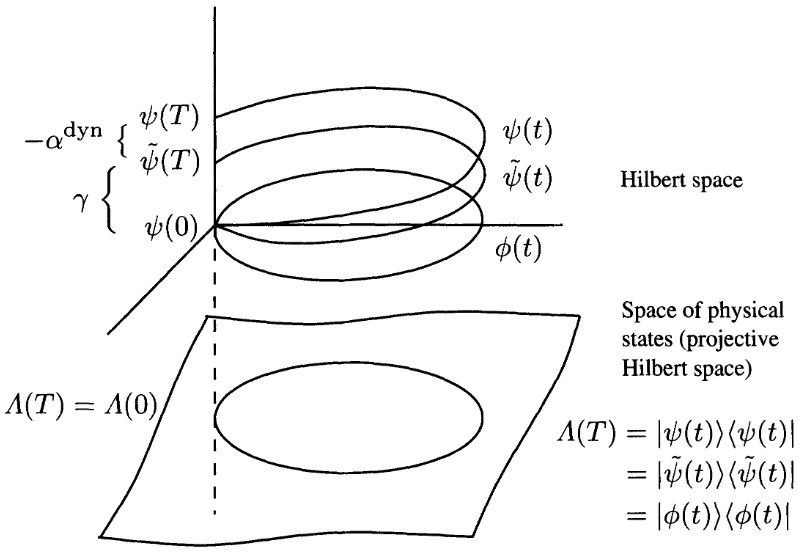
\includegraphics[width=0.7\textwidth]{fig/schéma2Bohm}
	\caption{Schéma de Bohm \cite{bohm_geometric_2003} sur les trois phases}
	\label{fig:2lifts}
\end{figure}

Quand on dit que $\Tilde{\psi}$ est l'\textit{horizontal lift}, on sous entend que le fibré est munie d'une connexion. Suivant l'approche quantique, elle est de la forme :
\[\forall \eta\in\Gamma(\mathcal{M}),\quad  \mathcal{A} \defeq \int_\gamma \big\langle \eta, h(\eta) \big\rangle\]
où $h$ est l'Hamiltonien de l'équation de Schrödinger (dont $\psi$ est supposé solution) :
\begin{equation}\label{eq:schrodinger}
	i\frac{d}{dt} \psi(t) = h\big(\psi(t)\big)
\end{equation}
Mais on a le choix de $h$. En particulier, si on veut pas de contrainte, on peut toujours poser :
\[h = i\frac{d}{dt}\]
Est-ce qu'on a le droit ? (je vois pas pourquoi on pourrait pas) Et si on le fait, qu'est-ce que ca dit du point de vue mécha Hamiltonienne ? (\apriori~rien vue l'EDP)
\\
Aussi, du pvd calculatoire / de la phase g, qu'est-ce qu'il se passe ? Typiquement, est-ce que y'a $\Tilde{\psi}$ devient un $\phi$ ?
\\

Aussi, chose remarquable, le fait que la phase géométrique soit invariante par gauge transfo réapprait dans le fait que $\phi$ ne soit pas définie à gauge tranfo près (sauf au bord). Par contre c'est étrange que 



\subsection{La vision Mukunda \& Simon \cite{mukunda_quantum_1993,mukunda_quantum_1993-1}}

\begin{itemize}
	\item Mukunda \& Simon\cite[p. 10]{mukunda_quantum_1993} partent des matrices de corrélation $\rho = \psi\psi^\dagger$ vérifiant (cas normé, p.50 pour le cas générale) :
	\begin{align*}
		\rho &= \rho^\dagger \geq 0  &  \rho^2 &= \rho  &  \tr(\rho) &= 1 (=\|\rho\|^2)
	\end{align*}
	et pose l'Hamiltonien  (resp. l'énergie kiné) :
	\begin{align*}
		H &= i\big( \dot{\psi} \psi^\dagger - \psi\dot{\psi}^\dagger - \langle \psi, \dot{\psi}\rangle\big)  &  \text{resp. }\ K &= \frac{d}{dt}\big( \psi\psi^\dagger \big) = \dot{\rho}
	\end{align*}
	qui donne :
	\[\frac{d}{dt}\psi = -i H\psi = \big( K + \langle\psi, \dot{\psi}\rangle \big)\]
	$K$ est "mieux" dans le sens où il est invariant par gauge-t. Aussi, comme c'est une dérivée d'une hermitienne elle est... hermitienne ? (mmmh).
	
	Anyway, on peut poser avec la bonne gauge :
	\[\frac{d}{dt}\Tilde{\psi} = K\Tilde{\psi}\]
	\\
	
	\item Voir page 20 pour passer de $\phaseg$ au Birgmann invar
	\\
	
	\item La phase totale $\phaset(\psi,t_0,t)$ est la phase dyn de la géodésique reliant $\psi(t)$ à $\psi(t_0)$ (ca commute ? surement pas)
	\\
	En somme, la phase totale est complètement indépendante du chemin $\psi$, ce qui est rassurant puisque c'est ce qu'on attend la phase totale : qu'elle ne compare que les états $\psi(t_0)$ et $\psi(t)$.
	
	\item L'invariant de Birgmann à des propriétés sommatoires similaires à un calcul de volume... transition parfaite vers la formule de Stokes !!!
	
	\item SUPER IMPORTANT : \cite[(8.6),p.51]{mukunda_quantum_1993} pour l'originie/choix de $\phaseg$ !
\end{itemize}




 


\section{Intuition sur les fondamentaux}

\subsection{Réflexion autour du produit hermitien}

Soit $x,y\in\C^n$ des vecteurs complexes et $X,Y\in\R^{2\times n}$ leur versions réelles. On note $x^j$ sa $j^{eme}$ composante complèxe et $x_1$ (resp. $x_2$) le vecteur composé de ses parties réelles (resp. imaginaires) :
\[x = \big(x^j\big)_j =  x_1 + ix_2 =  \big(x^j_1\big)_j +i \big(x^j_2\big)_j\]
\\
On a deux façon d'écrire le produit hermitien (canonique) de $x$ avec $y$.
\\
La première :
\begin{align*}
\langle x,y \rangle = \langle x_1 + ix_2, y_1 + iy_2\rangle &= \langle x_1, y_1\rangle - i \langle x_1,y_2\rangle +i\langle x_2, y_1\rangle + \langle x_2, y_2\rangle  \\
&= \langle x_1, y_1\rangle + \langle x_2, y_2\rangle 
+ i\big(\langle x_2, y_1\rangle - \langle x_1,y_2\rangle\big) \\
&= \sum_j x^j_1 y^j_1+ x^j_2 y^j_2
+ i\left(\sum_j x^j_2 y^j_1 -  x^j_1y^j_2\right) \\
&= \left\langle \begin{pmatrix} x_1 \\ x_2 \end{pmatrix},\begin{pmatrix} y_1 \\ y_2 \end{pmatrix}\right\rangle
+ i\left\langle \begin{pmatrix} x_1 \\ x_2 \end{pmatrix},\begin{pmatrix} -y_2 \\ y_1 \end{pmatrix}\right\rangle \\
&= \Big\langle X,Y\Big\rangle 
+ i\left\langle X,\begin{pmatrix} 0 & -I_n \\ I_n & 0 \end{pmatrix}\begin{pmatrix} y_1 \\ y_2 \end{pmatrix}\right\rangle\\
&= \Big\langle X,Y\Big\rangle 
- i\left\langle X,\begin{pmatrix} 0 & I_n \\ -I_n & 0 \end{pmatrix}Y\right\rangle
\end{align*}
\\
Cette formule peut s’interpréter en disant que le produit hermitien encode le produit scalaire entre $X$ et $Y$ et le produit scalaire de $X$ avec les vecteurs $y^j=(y^j_1, y^j_2)$  auquel on aurait applique une rotation de $90^\circ$ (rotation qui, par ailleurs, correspond à la multiplication par $i$ dans le plan complexe). Moralement, $\langle x,y \rangle =0$ demande une orthogonalité de $X$ à un plan, ce qui fait sens puisque cela tient compte du fait que les $x^j, y^j$ sont complexes (donc de dimension 2 en tant que $\R-$e.v.).
\\
Pour les connaisseurs, on retrouve l'égalité ``produit hermitien $=$ produit scalaire $-i$ forme symplectique'' !!
Voir
\href{https://fr.wikipedia.org/wiki/Espace_projectif#Espace_projectif_complexe}{plan proj complexe} et \href{https://fr.wikipedia.org/wiki/Vari%C3%A9t%C3%A9_k%C3%A4hl%C3%A9rienne}{variété kählérienne }
\\

On a aussi l'écriture (quand-même moins clair) :
\begin{align*}
\langle x,y \rangle &= \langle x_1, y_1\rangle + \langle x_2, y_2\rangle 
+ i\big(\langle x_2, y_1\rangle - \langle x_1,y_2\rangle\big) \\
&= \sum_j x^j_1 y^j_1+ x^j_2 y^j_2+ i\sum_j \big( x^j_2 y^j_1 - x^j_1y^j_2 \big) \\
&= \sum_j \big\langle X^j,Y^j\big\rangle - i\sum_j \det(X^j, Y^j)
%&= \sum_j \|X^j\|\|Y^j\| \cos \widehat{X^j,X^j} + i\sin \widehat{X^j,Y^j}
\end{align*}
Cette formule dit que les parties reélles et imaginaires du produit $\langle x,y \rangle$ encodent respectivement ``l'orthogonalité moyenne'' et la ``linéarité moyenne ''entre les familles de vecteurs $X^j\in\R^2$ et $Y^j\in\R^2$. L'orthogonalité d'une part parce que le produit scalaire s'annule en cas d'orthogonalité (no shit), la linéarité d'autre part car le déterminant s'annule en cas de colinéarité et moyenne car se sont des sommes sur $j$. \textbf{$\bf{\langle x,y \rangle=0}$ ne dit pas que les le vecteurs sont à la fois colinéaire et orthogonaux parce que ce sont des valeurs moyennes (\ie~annuler une somme ne veut pas dire que chacun des termes sont nuls).}
\\

Si maintenant on s'intéresse au cas $y=x$, on a $\forall h\in\C^n$ :
\begin{align*}
\langle x+h, x+h \rangle = \langle x, x \rangle + \langle x, h \rangle + \langle h, x \rangle + \langle h, h \rangle 
&= \langle x, x \rangle + \langle x, h \rangle  + \congu{\langle x, h \rangle }+ \langle h, h \rangle \\
&= \langle x, x \rangle + 2\Re e \langle x, h \rangle + \langle h, h \rangle
\end{align*}
Donc si $x\in\C^n$ est fonction d'un paramètre $t$, l'égalité $\ \langle x, \dot{x} \rangle = \frac{1}{2}\partial_t\langle x, x \rangle\ $ du cas réel devient :
\begin{equation}\label{eq:x_scal_dotx}
\langle x\,|\, \dot{x} \rangle = \frac{1}{2}\partial_t\langle x\,|\, x \rangle + i\left\langle X\,´\Big|\,\begin{pmatrix} 0 & -I_n \\ I_n & 0 \end{pmatrix}\dot{X}\right\rangle
\end{equation}
\\
En particulier, quand bien-même $x$ serait de norme constante, on aurait toujours un degré de liberté pour $\ \langle x, \dot{x} \rangle$ :
\[\|x\|=c\quad \Lr\quad \langle x, \dot{x} \rangle = i\left\langle X,\begin{pmatrix} 0 & -I_n \\ I_n & 0 \end{pmatrix}\dot{X}\right\rangle\]




\section{Description des signaux multivariés}\label{sec:bases}

\subsection{Cas bivarié et trivarié}

\subsubsection{Bivarié}

\begin{itemize}
	
	\item Avec la transformation :
	\[\bf{x} \leadsto \big(e^{i\phi}, \bf{x}\bf{x}^\dagger\big)\in\U{1}\times \PC{1}-ish\]
	On a :
	\begin{align*}
		\bf{x}\bf{x}^\dagger &= \frac{1}{2}\sum_{n=1}^3 S_i(t)\sigma_i  &  \left\{\begin{aligned}
			S_0(t) &=\, ^t\bf{x}\congu{\bf{x}} = \|\bf{x}\|^2 \\
			S_1(t) &= S_0(t) \cos 2\chi(t)\cos 2\theta(t)\\
			S_2(t) &= S_0(t) \cos 2\chi(t)\sin 2\theta(t)\\
			S_3(t) &= S_0(t) \sin 2\chi(t)
		\end{aligned} \right.
	\end{align*}
	
	\item En version quaternion ($\bf{j}$ fait office de $i$) \cite{lefevre_polarization_2021} :
	\begin{equation}
		\sa{\bf{x}} = a(t)e^{\bf{i}\theta} e^{-\bf{k}\chi} e^{\bf{j}\phi}
	\end{equation}
	Et les Stokes parameters sont donnée par :
	\[\sa{\bf{x}} \bf{j} \congu{\sa{\bf{x}}} = S_0  +\bf{i}S_3 + \bf{j}S_1 + \bf{k}S_2\]
	Et le lien avec les $\sigma_i$ se fait via (mais du coup les notations colles par :/) :
	\[(\sigma_0, \sigma_1, \sigma_2, \sigma_3) \leadsto (1, \bf{i}, \bf{j}, \bf{k})\]
	
	\item Et en version matrice de Pauli :
	\begin{equation}
		\sa{\bf{x}} = a(t)e^{i\phi} e^{i\theta \sigma_2} e^{-i\chi \sigma_1} \begin{pmatrix} 1 \\ 0 \end{pmatrix}
	\end{equation}
\end{itemize}
\noindent
Plus de détail : \\ 

On a un signal bivarié $\bf{x}(t) = \big(x(t),y(t)\big)$ qu'on transforme (voir \cref{subsec:transfo_SA}) soit la forme :
\[\sa{\bf{x}}(t) = \begin{pmatrix}x_+(t) \\ y_+(t)\end{pmatrix} = \begin{pmatrix}a_x(t) e^{i\phi_x(t)} \\ a_y(t) e^{i\phi_y(t)}\end{pmatrix}\in\C^2\]
\\

\`A côté de ça, on a les ellipses modulées :
\[z(t) = e^{i\theta}\big(a(t)\cos\phi(t) + ib(t) \sin\phi(t)\big) = a(t) e^{i\theta} \big( \sin\chi(t) \cos\phi(t) + i\sin\chi(t) \sin\phi(t) \big) \in\C\]
Qui sous forme vectoriel se réécrit \textbf{(pourquoi ???)} :
\begin{equation}%\label{eq:exp_elliptik}
	z(t) = e^{i\phi(t)} R_{\theta(t)}\begin{pmatrix} a(t) \\ -ib(t) \end{pmatrix} = a(t)e^{i\phi(t)} R_{\theta(t)} \begin{pmatrix} \cos\chi(t) \\ -i\sin\chi(t) \end{pmatrix} \in\C^2,\qquad R_\theta\in\SO_2(\R) \
\end{equation}
\\

Pour avoir la désinscription de $\bf{x}$ en terme d’ellipse, il suffit donc de poser :\footnote{C'est la version analytique du la version vectorielle de l'ellipse !}
\[\sa{\bf{x}}(t) = z(t)\quad \Llr\quad \begin{pmatrix}a_x(t) e^{i\phi_x(t)} \\ a_y(t) e^ {i\phi_y(t)}\end{pmatrix} = A(t)e^{i\phi} R_{\theta(t)} \begin{pmatrix} \cos\chi(t) \\ -i\sin\chi(t) \end{pmatrix}\]
\\
Ensuite, on pose :
\[\begin{pmatrix}z_+ \\ z_-\end{pmatrix} = \begin{pmatrix}a_+ e^{i\phi_+} \\ a_- e^{i\phi_-}\end{pmatrix} = \frac{1}{2}\begin{pmatrix}x_+ + iy_+ \\ x_+ - iy_+\end{pmatrix} = \frac{1}{2}\begin{pmatrix}1 & i \\ 1 & -i\end{pmatrix} \begin{pmatrix}x_+ \\ y_+\end{pmatrix}\]
\\
Et on a :
\begin{align*}
	2\phi &= \phi_+ + \phi_-  &  a &= A\cos\chi = a_+ + a_- \\
	2\theta &= \phi_+ - \phi_-  &  b &= A\sin\chi = a_+ - a_- 
\end{align*}
et on en déduit :
\begin{align*}
	A &= \sqrt{(a_+ + a_-)^2 + (a_+ - a_-)^2}  &  \begin{aligned} \cos\chi &= \frac{a_+ + a_- }{\sqrt{(a_+ + a_-)^2 + (a_+ - a_-)^2}}  \\  \sin\chi &= \frac{a_+ - a_- }{\sqrt{(a_+ + a_-)^2 + (a_+ - a_-)^2}}	\end{aligned}
\end{align*}
Ce qui donne \infine (super osef) :
\[\begin{pmatrix}x_+ \\ y_+\end{pmatrix} = e^{i\frac{\phi_+ + \phi_-}{2}} R_{\frac{\phi_+ - \phi_-}{2}} \begin{pmatrix}a_+ + a_- \\ -i(a_+ - a_-)\end{pmatrix}\]
\\

L'\cref{eq:exp_elliptik_2var} ce généralise  très bien, il suffit d'augmenter la taille de $R_\theta\in\SO_n(\R)$ et de lui donner le vecteur étendu :\footnote{\textit{Sachant que le vecteur contenant $a$ et $b$ est principalement nul, on peut réécrire le produit ne considérant que les deux premières colonnes de $R_\theta$.}}
\[z_x(t) = \begin{pmatrix}x_{1+}(t) \\ \vdots \\ 
	x_{n+}(t)\end{pmatrix} = e^{i\phi} R_{\theta(t)}\begin{pmatrix} a(t) \\ -ib(t) \\ 0 \\ \vdots \\ 0 \end{pmatrix} = A(t)e^{i\phi} R_{\theta(t)} \begin{pmatrix} \cos\chi(t) \\ -i\sin\chi(t) \\ 0 \\ \vdots \\ 0 \end{pmatrix}\]
\\

Maintenant, la question est de savoir comment généraliser la transformation en $(z_+, z_-)$ pour obtenir les paramètres $(A, \phi, R_\theta, \chi)$ dans ce cas...
\\
Pour généraliser le procédé, on peut noter que :
\[\begin{pmatrix}z_+ \\ z_-\end{pmatrix} = \frac{1}{2}\begin{pmatrix}1 & i \\ 1 & -i\end{pmatrix} \begin{pmatrix}x_+ \\ y_+\end{pmatrix} = \frac{1}{\sqrt{2}}U \begin{pmatrix}x_+ \\ y_+\end{pmatrix}\qquad\qquad \text{avec }\ U=\frac{1}{\sqrt{2}}\begin{pmatrix}1 & i \\ 1 & -i\end{pmatrix}\in\U{2}\]
\\ 
Ce qui ramène à se demander comment généraliser $U$ à $\U{n}$. Le problème est que $U$ est indépendant de tout les paramètres $(A, \phi, R_\theta, \chi)$ et sa généralisation est vraiment pas évidente sachant qu'on que le formule avec $n=2$... et pour $n=3$ ca devient déjà chaud (pour rappelle $\dim \SO_n(\R)=\frac{n(n-1)}{2}$ et donc $\theta\in\R^n$, ce qui rend le problème de pire en pire à mesure qu'on augmente $n$).



\subsubsection{Trivarié}

\begin{itemize}
	\item Version de Lilly \cite{lilly_modulated_2011}
	\begin{equation}
		\begin{aligned}
			\sa{\bf{x}}(t) &= e^{i\phi(t)} R_1\big(\alpha(t)\big)\ R_3\big(\beta(t)\big)\ R_1\big(\theta(t)\big)\begin{pmatrix}
				a(t) \\ -ib(t) \\ 0
			\end{pmatrix} \\
			&= a(t)e^{i\phi(t)} R_1\big(\alpha(t)\big)\ R_3\big(\beta(t)\big)\ R_1\big(\theta(t)\big)\begin{pmatrix}
				\cos\chi(t) \\ -i\sin\chi(t) \\ 0
			\end{pmatrix}
		\end{aligned}
	\end{equation}
	
	\begin{align*}
		&\text{avec : }  &  
		R_1(\theta) &= \begin{pmatrix}
			1 & 0 & 0 \\ 0 & \cos\theta & -\sin\theta \\ 0 & \sin\theta & \cos\theta
		\end{pmatrix}  &  
		R_3(\theta) &= \begin{pmatrix}
			\cos\theta & -\sin\theta & 0 \\ \sin\theta & \cos\theta & 0 \\ 0 & 0 & 1 
		\end{pmatrix}
	\end{align*}
	
	Donc une amplitude / phase instantanée $A$ / $\phi$ et une polarisation instantanée d'ellipse paramétrée par $\chi$ et orientée par la rotation $R_1R_3R_1$.
	
	\item On note d'abord que (Lefevre \cite{lefevre_polarization_2021}) :
	\[\begin{pmatrix}
		\cos\chi(t) \\ -i\sin\chi(t) \\ 0
	\end{pmatrix} = \begin{pmatrix}
		\cos\chi(t) & i\sin\chi(t) & 0 \\ -i\sin\chi(t) & \cos\chi(t) & 0 \\ 0 & 0 & 1
	\end{pmatrix}\begin{pmatrix}
		1 \\ 0 \\ 0
	\end{pmatrix}\]
	Ce qui, en terme de matrice de Gall-man $(\lambda_i)$ (généralisation de la base de Pauli à $\U{3}$), devient :
	\begin{align*}
		\sa{\bf{x}}(t) &= a(t)e^{i\phi(t)} R_1\big(\alpha(t)\big)\ R_3\big(\beta(t)\big)\ R_1\big(\theta(t)\big)\begin{pmatrix}
			\cos\chi(t) \\ -i\sin\chi(t) \\ 0
		\end{pmatrix} \\
		&= a(t)e^{i\phi(t)} e^{i\alpha \lambda_7} e^{i\beta \lambda_3} e^{i\theta \lambda_7} e^{-i\chi \lambda_1}\begin{pmatrix}
			1 \\ 0 \\ 0
		\end{pmatrix}
	\end{align*}
\end{itemize}



\subsection{Mon blabla}\label{subsec:blabla}


\begin{proposition}\label{prop:quatern}
Les signaux bivariés se décrivent très simplement à l'aide des quaternions. En considérant $\{1, \bf{i},\bf{j},\bf{k}\}$ la base canonique des quaternions $\mathbb{H}$, on peut voir $\psi$ comme étant à valeur dans ${\C_{\bf{j}}}^n$ ($\C_{\bf{j}} :=\R\times \bf{j}\R$), de sorte que :
\[\forall \psi\in L^2(\R,\mathbb{H}),\ \exists a,\theta,\chi,\varphi \in\mathcal{C}(\R)\ |\quad \psi(t) = a(t)e^{\bf{i}\theta(t)}e^{-\bf{k}\chi(t)}e^{\bf{j}\varphi(t)}\]
\\
Sous cette forme, les paramètres $a$ et $\varphi$ s'interprètent respectivement comme l'amplitude et la phase instantanée du signal. Les deux paramètres restant contrôle l'ellipticité ($\chi$) et l'orientation ($\theta$) de l’ellipse de polarisation instantanée. C'est-à-dire l'ellipse que suit la signal à l'instant $t$.
\\
Dit autrement, à tout instant $t$, $\psi(t)$ est vu comme une point d'une ellipse dont la taille est caractériser par $a(t)$, l'ellipticité par $\chi(t)$ et l'orientation par $\theta(t)$. $\phi(t)$ permet lui de situer $\varphi(t)$ sur cette ellipse.
\\

\textit{Le problème de cette représentation est qu'elle se généralise mal aux signaux plus que $2-$variés et, à notre connaissant, il n'existe pas d'extensions des quaternions à de plus haute dimension. voir \cref{prop:gene_param_signal_v1,prop:gene_param_signal_v2}, \cref{eq:phase_tot,,eq:phase_dyn,eq:phase_geo}} 
\end{proposition}

Il est évident que cette représentation est présent bien plus de paramètre que nécessaire, puisse que deux devrait suffire. Pour autant, elle permet de mieux \textbf{je sais quoi mais c'est sur qu'il y'a une raison}.
\\
Si cette représentation se généralise mal parce qu'elle demanderait d'avoir une extension de $\mathbb{H}$, sont interprétations graphique, elle, se généralise très bien. Par exemple, en dimension 3, alors l'ellipse devient une ellipsoïde. L'amplitude reste de dimension 1 parce qu'elle ne fait que contrôler la taille de cet ellipsoïde, mais les autres paramètres eux doivent être de dimension 2. L'ellipsoïde à besoin de deux angles pour être orienté, possède deux degrés d'ellipticité et ces points sont déterminés par deux angles.


\begin{proposition}\label{prop:gene_param_signal_v1}
Plus généralement, tout signal multivarié $\psi$ est (\textit{devrait être}) caractérisé par quatre paramètres (donc $1+(n-1)(\frac{n}{2}-2)$ scalaires) :
\begin{align*}
	a&\in\mathcal{C}(\R,\R^+)  &  \theta&\in\mathcal{C}(\R, [-\pi/2,\pi/2]^{\frac{n(n-1)}{2}})  &  \chi&\in\mathcal{C}(\R, [-\pi/4,\pi/4]^{n-1})  &  \varphi&\in\mathcal{C}(\R, [-\pi,\pi]^{n-1})
\end{align*}	
\end{proposition}

\`A bien y réfléchir, décrire un ellipsoïde dans l'espace, c'est exactement de que font les matrices symétriques définies positives. Donc on pourrait tout à fait remplacer les informations $(a,\theta,\chi)$ par une matrice symétrique positive de dimension $n$. Il ne resterait alors plus que $\varphi$ qui, de toute façon ne devrait pas trop être lié aux autres paramètres.

Enfin, surement que si parce que y'a un monde pour $\varphi=0_\R^n$ et c'est le reste des paramètres qui fait le travail. Mais clairement c'est pas intéressant comme description. L'idée serait plutôt décrire le signal $\psi$ en minimisant les variations de $(a,\theta,\chi)$.
Ca appelle clairement à chercher que dans l'espace de Siegel mais pas seulement, parce que c'est pas juste des chemins chez Siegel qui nous intéresse.

Ou alors c'est le jeu de gauge qui fait qu'on tue $\varphi$ ? auquel cas tout les jours Siegel.
\\

\textit{BTW, les quaternions c'est fait pour décrire les rotations et c'est (quasiment) ce qu'on fait avec, donc aller chercher dans un espace de matrices pour généraliser le principe c'est pas déconnant.}
\\
\textit{D'ailleurs, vu que c'est pas exactement ce qu'on fait avec, dans quelle mesure c'est pas le cas et est-ce qu'on exploite vraiment la structure des quaternions ?}


\begin{proposition}\label{prop:gene_param_signal_v2}
Autre approche : un signal multivarié étant moralement un chemin de $\R^n$, son graphe est une variété (plongée) de dimenion 1. Sachant cela, si en chaque instant on veut définir l'ellipsoïde sur laquelle elle repose à un insant $t$, il est morale que cette ellipsoïde soit en fait une ellipse puisque c'est elle-même une variété de dimension 1.
\\
Partant de là, on aurait toujours $a$, $\chi$ et $\phi$ pour la décrire et seulement $\theta$ gagnerait en dimension pour pouvoir orienter l'ellipse dans les $n$ axes. $\psi$ serait alors la données de $3+\frac{n(n-1)}{2}$ paramètres :
\begin{align*}
	a&\in\mathcal{C}(\R,\R^+)  &  \theta&\in\mathcal{C}(\R, [-\pi,\pi]^{\frac{n(n-1)}{2}})  &  \chi&\in\mathcal{C}(\R, [-\pi/4,\pi/4])  &  \varphi&\in\mathcal{C}(\R, [-\pi,\pi])
\end{align*}
\end{proposition}

On aurait beaucoup moins de paramètre et c'est quand-même bien. En même temps ca parait plus contraignant comme modèle. Pour comparer les deux, il faudrait voir comment les deux se décomposant dans le cas d'un signal qui ne varierait sur une ellipsoïde fixe. \ie dans un cas où $\theta,\chi$ de la \cref{prop:gene_param_signal_v1} varie pas alors que ceux de la \cref{prop:gene_param_signal_v2} si.



\section{Vrac}

\subsection{Random  stuff ready pour rédac (+labeled)}

\begin{definition}[Signal multivarié]\label{def:signal_multivar}
	Un \emph{signal multivarié}, ou \emph{$n-$varié}, est un vecteur composé de $n\in\N^*$ signaux $x_i$. Si $n=2$, alors on parle de signal \emph{bivarié}.
	\\
	Dans la continuité de ce qui à été dit dans la \cref{subsec:transfo_SA}, dans le cas des signaux réels, on s'intéressera au vecteur composé des transformées en SA (eq. \ref{eq:transfo_SA}, déf. \ref{def:transfo_sa&hilbert}) des $x_i$.
	\textbf{Au moins dans toute cette \namecref{sec:sign_multivar}}, un tel signal sera noté :
	\[\sa{x}(t)\ :\quad \begin{aligned} 
		\R\quad &\lr\qquad \C^n \\t\quad &\longmapsto\ \begin{pmatrix} \mathcal{A}[x_1] \\ 
			\mathcal{A}[x_2] \\ \vdots \\ \mathcal{A}[x_n] \end{pmatrix}
	\end{aligned} \]
	On supposera que chaque composante $x_i$ de $\bf{x}$ aura autant de régularité et de condition d'intégrabilité que nécessaire \textbf{(il vaudra préciser lesquelles à un moment)}.
\end{definition}

\begin{definition}\label{def:phase_dyn}
	Ainsi, il reste tout un degré de liberté au produit $\ \langle x, \dot{x} \rangle\ $ même si $x\in\S{2n}$. En intégrant ce degré de liberté supplémentaire, c'est-à-dire en tenant compte de son évolution sur la période $[t_0,t]$, l'on obtient ce qui est appeller le \emph{phase dynamique} :
	\[\phased \defeq \phased(t_0,t) = \int_{t_0}^t \Im m \big\langle \psi(s) \, |\, \dot{\psi}(s) \big\rangle ds\]
	Elle dynamique en cela qu'elle est propre au variation de $\psi$ et qu'elle considère tout l'évolution de $\psi$ : ça dynamique.
\end{definition}


\begin{definition}[Connexion de Berry]\label{def:berry_connx}
	On appelle \emph{connexion de Berry} le champ de forme linéaire :
	\begin{equation}\label{eq:berry_connx}
		\forall \psi\in\mathpzc{M},\quad A_\psi :\ \begin{aligned} T_\psi\mathpzc{M}\ &\lr\qquad\ \R \\ \phi\quad &\longmapsto\ \Im m \big\langle \psi(s) \, |\, \phi(s) \big\rangle
		\end{aligned}
	\end{equation}
	\textbf{Elle a rien d'une connexion par contre :/}
\end{definition}



\subsection{Bilan des formules}

\begin{itemize}
	\item Les phases de $\psi$ entre les instants $t_0$ et $t$ :
	\begin{equation}\label{eq:phase_tot}
		\phaset(\psi, t_0, t) \defeq \arg\big\langle\psi(t_0) \,|\, \psi(t)\big\rangle = \arctan \left( -\frac{\big\langle\psi(t_0), \omega\psi(t)\big\rangle}{\big\langle\psi(t_0), \psi(t)\big\rangle} \right)
	\end{equation}
	
	\begin{equation}\label{eq:phase_dyn}
		\phased(\psi,t_0,t) \defeq \Im m \int_{t_0}^t\big\langle \psi(s) \,|\, \dot{\psi}(s) \big\rangle ds
	\end{equation}
	
	\begin{equation}\label{eq:phase_geo}
		\phaseg(\psi, t_0, t) \defeq \phaset(\psi, t_0, t) - \phased(\psi,t_0,t)
	\end{equation}
	
	\item (conservative) Équation Schrödinger et de Liouville-von Neumann ($h(R)$ : Hamiltonien des paramètres $R$, $W$ : opérateurs statistique ) \cite[p.6]{bohm_geometric_2003} :
	\begin{equation}%\label{eq:schrodinger}
		i\frac{d \psi(t)}{dt} = h(R)\psi(t)
	\end{equation}
	\begin{equation}\label{eq:liouville-neumann}
		i\frac{d W(t)}{dt} = \big[h(R),W(t)\big] \qquad\qquad [\cdot\,,\cdot]=\text{ commutateur ?}
	\end{equation}
	
	\item Moment angulaire (viteuf) $\forall z\in\C$ :
	\begin{equation}\label{eq:mom_angu}
		M(t) = \Re e \big(iz\congu{z}'\big) = -\Im m z\congu{z}'  \qquad\qquad \text{thoughts ?}
	\end{equation}
	
\end{itemize}


\subsection{Thoughts}

\begin{itemize}
	\item Si la phase géo est la phase dyn - phase tot et est invariante as gauge t, est-ce que la phase tot correspond à la phase (dyn) entre $t_0$ et $t$ suivant la géodesique ?
	
	\item La ``Berry connection'' c'est une vraie connexion ? elle est où la covariance alors ?
\end{itemize}

\[\underline{\overline{\qquad\qquad\qquad\qquad\qquad\qquad\qquad\qquad\qquad\qquad\qquad\qquad\qquad\qquad\qquad\qquad\qquad\qquad}}\]{\color{white}relbinrei}

\begin{itemize}
	\item ``horizontal lift'' : pourquoi horizontal ? en quel sens ? (parce que fibré)
	
	\item Fréquence de Rubi
	
	\item Matrice/base de Pauli et généralisation, groupe $SU(n)$ (un peu de quantique ?)
	
	\item Monopole de Dirac + lien avec la phase géo (un peu d'électro-magnétisme ?)
	
	\item Invariant de Bargmann + série de Dyson
\end{itemize}
